% This file was created by matlab2tikz.
%
%The latest updates can be retrieved from
%  http://www.mathworks.com/matlabcentral/fileexchange/22022-matlab2tikz-matlab2tikz
%where you can also make suggestions and rate matlab2tikz.
%
\definecolor{mycolor1}{rgb}{0.06600,0.44300,0.74500}%
\definecolor{mycolor2}{rgb}{0.12941,0.12941,0.12941}%
\definecolor{mycolor3}{rgb}{0.86600,0.32900,0.00000}%
\definecolor{mycolor4}{rgb}{0.92900,0.69400,0.12500}%
\definecolor{mycolor5}{rgb}{0.52100,0.08600,0.81900}%
\definecolor{mycolor6}{rgb}{0.23100,0.66600,0.19600}%
\definecolor{mycolor7}{rgb}{0.18400,0.74500,0.93700}%
\definecolor{mycolor8}{rgb}{0.81900,0.01500,0.54500}%
%
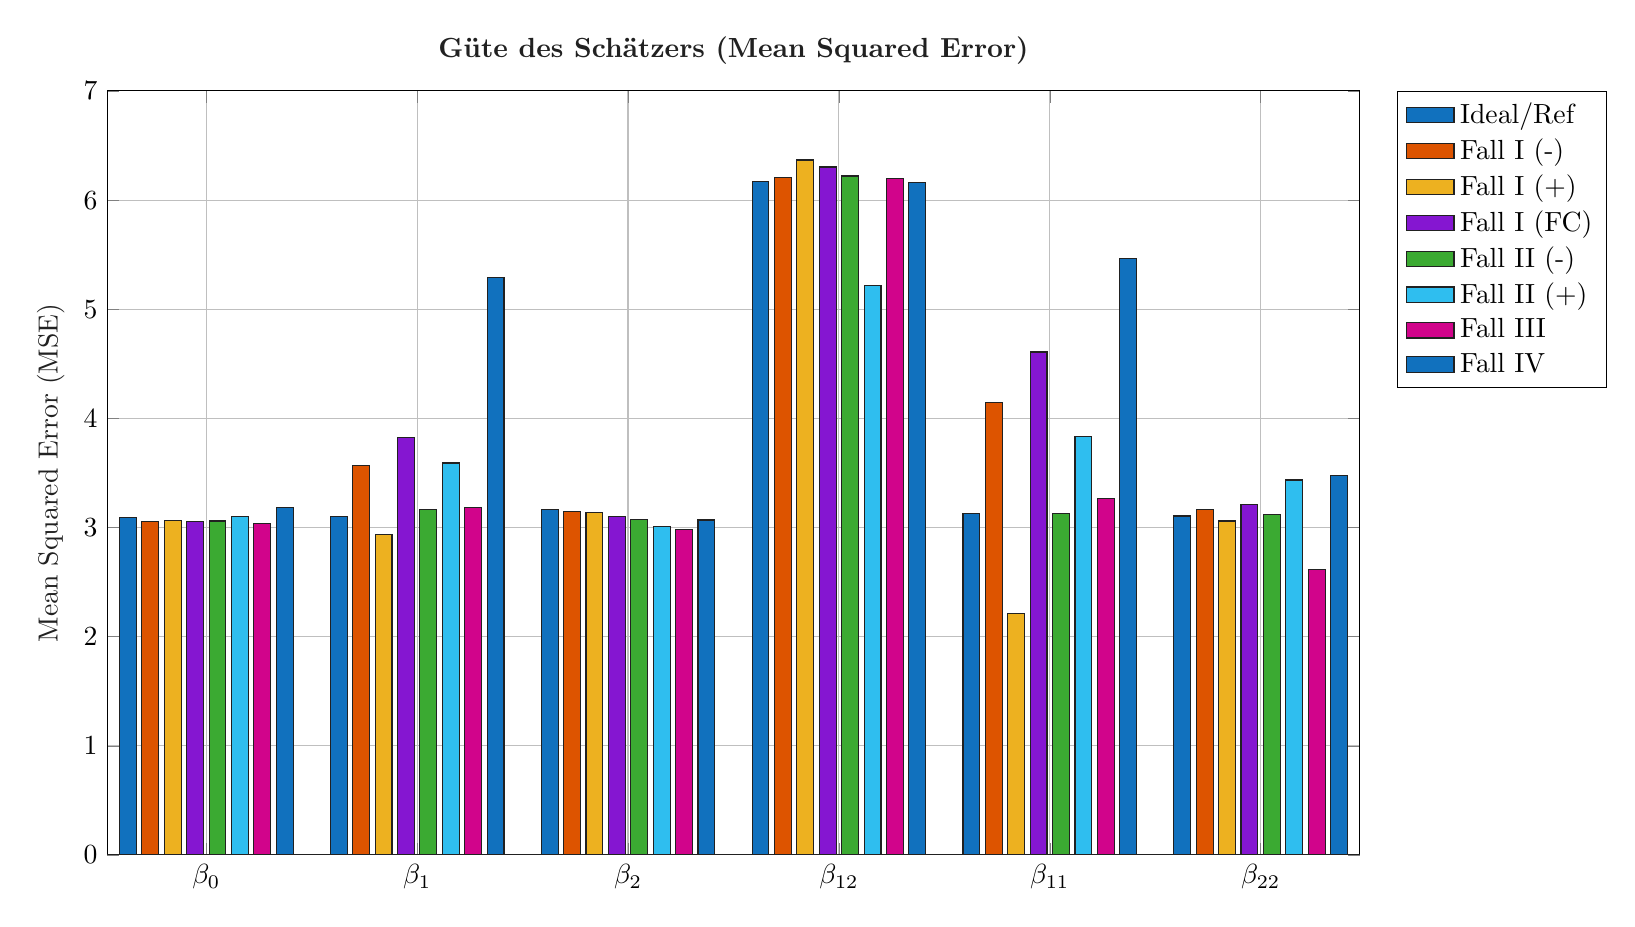
\begin{tikzpicture}

\begin{axis}[%
width=6.263in,
height=3.82in,
at={(1.051in,0.516in)},
scale only axis,
bar shift auto,
xmin=0.53,
xmax=6.47,
xtick={1,2,3,4,5,6},
xticklabels={{$\beta_0$},{$\beta_1$},{$\beta_2$},{$\beta_{12}$},{$\beta_{11}$},{$\beta_{22}$}},
ymin=0,
ymax=7,
ylabel style={font=\color{mycolor2}},
ylabel={Mean Squared Error (MSE)},
axis background/.style={fill=white},
title style={font=\bfseries\color{mycolor2}},
title={\textbf{Güte des Schätzers (Mean Squared Error)}},
xmajorgrids,
ymajorgrids,
legend style={at={(1.03,1)}, anchor=north west, legend cell align=left, align=left}
]
\addplot[ybar, bar width=0.08, fill=mycolor1, draw=mycolor2, area legend] table[row sep=crcr] {%
1	3.08944168696625\\
2	3.09759791290986\\
3	3.16642316783376\\
4	6.1732490235233\\
5	3.1268860126307\\
6	3.10533664231659\\
};
\addplot[forget plot, color=mycolor2] table[row sep=crcr] {%
0.53	0\\
6.47	0\\
};
\addlegendentry{Ideal/Ref}

\addplot[ybar, bar width=0.08, fill=mycolor3, draw=mycolor2, area legend] table[row sep=crcr] {%
1	3.05188820686549\\
2	3.56874598638153\\
3	3.14728213165307\\
4	6.2034914985615\\
5	4.14589057163559\\
6	3.16679348236323\\
};
\addplot[forget plot, color=mycolor2] table[row sep=crcr] {%
0.53	0\\
6.47	0\\
};
\addlegendentry{Fall I (-)}

\addplot[ybar, bar width=0.08, fill=mycolor4, draw=mycolor2, area legend] table[row sep=crcr] {%
1	3.06683624859833\\
2	2.93898766902387\\
3	3.14116701287003\\
4	6.36681912548429\\
5	2.21384879588605\\
6	3.05965090223526\\
};
\addplot[forget plot, color=mycolor2] table[row sep=crcr] {%
0.53	0\\
6.47	0\\
};
\addlegendentry{Fall I (+)}

\addplot[ybar, bar width=0.08, fill=mycolor5, draw=mycolor2, area legend] table[row sep=crcr] {%
1	3.056663049461\\
2	3.82489200875607\\
3	3.09704692053109\\
4	6.30307291239627\\
5	4.60852130621545\\
6	3.2103078490063\\
};
\addplot[forget plot, color=mycolor2] table[row sep=crcr] {%
0.53	0\\
6.47	0\\
};
\addlegendentry{Fall I (FC)}

\addplot[ybar, bar width=0.08, fill=mycolor6, draw=mycolor2, area legend] table[row sep=crcr] {%
1	3.05947030395935\\
2	3.16673029976763\\
3	3.06947673638661\\
4	6.2208133646178\\
5	3.13216058942208\\
6	3.1193558849623\\
};
\addplot[forget plot, color=mycolor2] table[row sep=crcr] {%
0.53	0\\
6.47	0\\
};
\addlegendentry{Fall II (-)}

\addplot[ybar, bar width=0.08, fill=mycolor7, draw=mycolor2, area legend] table[row sep=crcr] {%
1	3.09939564156352\\
2	3.59092092242696\\
3	3.01304355503128\\
4	5.21495790297925\\
5	3.83127096488266\\
6	3.43521646445687\\
};
\addplot[forget plot, color=mycolor2] table[row sep=crcr] {%
0.53	0\\
6.47	0\\
};
\addlegendentry{Fall II (+)}

\addplot[ybar, bar width=0.08, fill=mycolor8, draw=mycolor2, area legend] table[row sep=crcr] {%
1	3.03785277070444\\
2	3.17999645981296\\
3	2.98411315433579\\
4	6.19906815648671\\
5	3.26925143508281\\
6	2.61727949484879\\
};
\addplot[forget plot, color=mycolor2] table[row sep=crcr] {%
0.53	0\\
6.47	0\\
};
\addlegendentry{Fall III}

\addplot[ybar, bar width=0.08, fill=mycolor1, draw=mycolor2, area legend] table[row sep=crcr] {%
1	3.18279613996327\\
2	5.29290915568838\\
3	3.06913135117923\\
4	6.16508134053124\\
5	5.46332908246198\\
6	3.47264711639212\\
};
\addplot[forget plot, color=mycolor2] table[row sep=crcr] {%
0.53	0\\
6.47	0\\
};
\addlegendentry{Fall IV}

\end{axis}
\end{tikzpicture}%